\chapter{Methodik}
\label{ch:methodik}

\section{LimeSurvey}

LimeSurvey ist ein von der gleichnamigen deutschen Firma entwickeltes Werkzeug für Umfragen.
Laut ihrer Website\cite{ls} ist LimeSurvey ein für Einsteiger und Profis, sowie für Privatpersonen als auch Institutionen gut geeignetes Werkzeug, um die Meinungen, Interessen und Entscheidungsgrundlagen einer Zielgruppe herauszufinden.
Es wird seit 2006 an der Software entwickelt und sie ist sowohl als Cloud-Edition über die Firma erhältlich, sowie auch als OpenSource-Projekt in der Community-Edition.\\

Falls man die Cloud-Edition nutzen will, hat man fünf Optionen: \textit{Free}, \textit{Basic}, \textit{Expert}, \textit{Enterprise} und \textit{Corporate}.
Diese unterscheiden sich vor allem durch die Zahl an Antworten pro Monat, die Menge an Upload-Speicher, E-Mail-Support, White-Label-Umfragen, Alias-Domains und die Entfernung des LimeSurvey-Brandings.
Innerhalb der \textit{Corporate}-Lösung kann man noch dedizierte Server und die Nutzung der Security Assertion Markup Language (SAML) beantragen.

\subsection{Community-Edition}

Zum Erstellen von Umfragen, welche in dieser Arbeit gebraucht werden, wird eine Version der Community-Edition genutzt (Version \jv{3.27.6}).
Diese nutzt Docker, um die Website möglichst separat vom restlichen System zu halten.
So muss man Abhängigkeiten nicht auf dem eigenen System installieren und verwalten.
Zur Verwaltung der Docker-Version des \enquote{Australian Consortium for Social \& Political Research Inc.} (ACSPRI) wird eine Docker-Compose-Datei genutzt, welche online zur Verfügung steht \cite{docker_comp}.

\subsection{Features}

Alle her aufgelisteten Informationen wurden der Dokumentation, dem LimeSurvey Manual\cite{lsm} entnommen.

\subsubsection{ExpressionScript}
\label{m:expr_script}
Mit Expression Script lässt sich komplexe Logik in eine Umfrage einbringen.
Die LimeSurvey-interne Skriptsprache lässt Bedingungen zu, unter denen bestimmte Fragen oder Antworten angezeigt werden sollen.
Man kann hier sowohl Antworten auf vorherige Fragen einbinden, als auch Informationen über den Teilnehmer, welche er vorher angegeben hat beziehungsweise welche über ihn gespeichert wurden.
Man kann mehrere Szenarios designen und es sind Vergleiche mit den Standard-Operatoren sowie RegEx möglich.

\subsubsection{Timings}

Es ist möglich, genau festzulegen, wie viel Zeit ein Nutzer zum Beantworten einer Frage hat.
Es können Warnmeldungen zu bestimmten Abschnitten innerhalb der Zeitperiode angezeigt werden, die CSS-Klasse, welche Aspekte der Darstellung einer Frage bestimmt, kann angepasst werden und das Beantworten anderer Fragen kann unterbunden werden.

\subsection{Fragegruppen}

Fragen in LimeSurvey sind in Fragegruppen unterteilt. Jede Frage ist genau einer Gruppe zugeordnet.
Eine Gruppe kann beliebig viele Fragen enthalten, weiterhin hat sie einen Titel, eine Beschreibung, eine Randomisierungsgruppe und eine Relevanz-Gleichung, wo mittels ExpressionScript (siehe \cref{m:expr_script}) angegeben werden kann, wann die Fragen dieser Gruppe angezeigt werden sollen.
Es darf beliebig viele Fragegruppen geben.

\subsection{Fragetypen}
\label{met:q_types}

Es gibt 36 Fragetypen in LimeSurvey, welche in fünf Kategorien unterteilt sind.
Davon sind allerdings nicht alle tatsächlich Fragen, auf die der Teilnehmer antworten kann, insgesamt gibt es vier Fragetypen, welche nicht explizit Fragen sind. %TODO: wirklich vier?
Die möglichen Antworten auf Freitext- und Zahlenfragen lassen sich mittels RegEx limitieren.
Es gibt pro Frage einen optionalen Hilfstext.
Fragen mit vordefinierten Antworten erhalten eine \enquote{Keine Antwort}-Option, wenn sie nicht verpflichtend sind.
Im folgenden werden alle Typen einmal aufgelistet und kurz beschrieben.


\subsubsection{Einfachauswahl}

Auf folgende Fragen kann man maximal eine Antwort geben.
\begin{description}
	\item[5 Punkte Wahl] Hier kann auf einer Skala von 1 bis 5 ein Wert ausgewählt werden.
	\item[Liste] Hier kann aus einer vordefinierten Liste eine Antwort gewählt werden. Es gibt drei unterschiedliche Darstellungsmöglichkeiten für diese Liste, entweder als Dropdown-Menü, als Bootstrap-Buttons oder mit Radio-Buttons neben den Antworten.
	\item[Liste mit Kommentar] Dies ist eine Listen-Frage wie oben, allerdings kann für die Frage auch noch ein Kommentar im Freitext geschrieben werden.
	\item[Image-Select-List] Hier wird zu der Liste an Antworten noch ein Bild angezeigt. Die Antworten werden mit Radio-Buttons daneben angezeigt.
\end{description}

\subsubsection{Matrix}

Pro Frage gibt es beliebig viele Subfragen, für jede Subfrage kann eine der vordefinierten Antworten ausgewählt werden.
Subfragen werden typischerweise als Zeilen dargestellt, die Antworten als Spalten.

\begin{description}
	\item[5 Punkte] Hier kann auf einer Skala von 1 bis 5 ein Wert ausgewählt werden.
	\item[10 Punkte] Hier kann auf einer Skala vom 1 bis 10 ein Wert ausgewählt werden.
	\item[Z/G/A] Hier kann aus den drei Möglichkeiten \enquote{Zunahme/Gleich/Abnahme} eine gewählt werden.
	\item[J/N/U] Hier kann aus den drei Möglichkeiten \enquote{Ja/Nein/Unsicher} eine gewählt werden.
	\item[Matrix (Custom)] Hier kann eine eigene Liste an Antwortmöglichkeiten definiert werden.
	\item[Matrix nach Spalte] Identisch zu Matrix (Custom), allerdings werden Zeilen und Spalten getauscht.
	\item[Dual Matrix] Es gibt zwei selbst erstellbare Listen an Antwortmöglichkeiten, man kann aus beiden eine Antwort pro Subfrage wählen.
	\item[Matrix (Freitext)] Hier kann man zwei Listen an Subfragen angeben. Daraus wird dann eine Matrix erstellt, wo in jeder Zelle Freitext als Antwort geschrieben werden kann.
	\item[Matrix (Zahlen)] Identisch zu Matrix (Freitext), aber es können nur Zahlen als Antwort angegeben werden.
\end{description}

\subsubsection{Multiple Choice}

Hier können mehrere Antworten aus einer vordefinierten Liste ausgewählt werden.
Optional kann ein \enquote{Anderes}-Feld zugänglich gemacht werden, in welches Teilnehmer eine eigene Antwort schreiben können.

\begin{description}
	\item[Multiple Choice] Darstellung als Bootstrap-Buttons oder Radio-List ist möglich.
	\item[Image Select] Hier wird ein Bild mit angezeigt.
	\item[Kommentar] Hier kann ein Kommentar pro Antwortfeld geschrieben werden.
\end{description}

\subsubsection{Textfragen}

\begin{description}
	\item[Browser Detect] Erkennt den Webbrowser des Teilnehmers. Dies ist keine Frage, welche der Teilnehmer beantworten kann.
	\item[Freitext] Hier kann der Teilnehmer einen Text eintippen. Es gibt kurze, lange und riesige Freitexte.
	\item[Mehrere Texte] Es gibt mehrere Subfragen. Für jede kann ein kurzer Freitext angegeben werden.
	\item[Input on Demand] Die Frage ist funktional identisch zu \el{Mehrere Texte}, allerdings muss der Teilnehmer einen Knopf drücken, um die nächste Subfrage angezeigt zu bekommen.
\end{description}

\subsubsection{Maskenfragen}

\begin{description}
	\item[Datum/Zeit] Hier kann ein Datum und eine Uhrzeit angegeben werden. Das Format ist einstellbar, es kann auch ein minimales Datum angegeben werden.
	\item[Ja/Nein] Hier kann mit Ja oder Nein geantwortet werden.
	\item[Gleichung] Bei diesem Typ werden Antworten auf vorher gestellte Fragen verwendet, um sie in einer Gleichung zu verarbeiten und das Ergebnis anzuzeigen.
	\item[Dateiupload] Hier kann eine Datei als Antwort hochgeladen werden.
	\item[Geschlecht] Hier kann zwischen \enquote{Männlich}, \enquote{Weiblich} und \enquote{Keine Antwort} ausgewählt werden.
	\item[Sprachumschaltung] Hier kann der Teilnehmer die Sprache ändern. Auch das ist keine richtige Frage.
	\item[Zahleneingabe] Hier kann nach einer Zahl als Antwort gefragt werden.
	\item[Mehrfache Zahlen] Hier gibt es mehrere Subfragen, auf die jeweils mit einer Zahl geantwortet werden muss. Die Maximal/Minimal-Werte sind limitierbar, genau so wie auch die Maximal- und Minimal-Summe. Es können genaue Gesamtergebnisse verlangt werden und nur Ganzzahlen als Antwort verlangt werden.
	\item[Ranking (Advanced)] Hier kann der Teilnehmer Elemente aus einer vordifinierten Liste sortieren. Es müssen nicht alle Elemente einsortiert werden.
	\item[Textanzeige] Hier wird ein Text angezeigt. Auch hier kann nicht geantwortet werden.
\end{description}

\subsection{Export}
\subsubsection{LimeSurvey Archiv}
\label{m:lsa}
Das LimeSurvey Archiv ist eine von sieben Möglichkeiten, Daten von einer LimeSurvey Umfrage zu exportieren.
Ein solches Archiv ist eine komprimierte Datei im .lsa-Format, welche mehrere extrahierbare Dateien enthält.
Die Zahl und Art der Dateien ist dabei abhängig von den Einstellungen. Zwei Dateien sind immer enthalten:

Die erste Datei enthält die Umfrage-Struktur sowie Informationen über die Art und Weise, wie die Fragen dargestellt werden sollen (die .lss-Datei).
Die zweite Datei enthält die Antworten der Teilnehmer (.lsr-Datei).
Ausdrücklich erwähnt wird dabei, dass Dateien, die als Antwort auf eine Frage hochgeladen wurden, nicht Teil des Archivs sind.
Eine weitere, optionale, Datei ist eine Token-Datei (.lst), welche nur enthalten ist, wenn mögliche Teilnehmer der Umfrage im Vorhinein festgelegt wurden.
Hier sind Informationen über den Teilnehmer gespeichert, in den Antworten wird pro Teilnehmer ein Token referenziert, sodass man die Antworten einem Teilnehmer zuordnen kann.

\subsubsection{Weitere Exportmöglichkeiten}
\begin{description}
	\item[LSS] Es ist möglich, nur die im LSA enthaltene LSS-Datei zu exportieren, das wird mittels dieser Option gemacht.
	\item[Excel/.csv] Hier sind weitere Einstellungen möglich, wie das Exportieren eines Teils der Antworten oder die Wahl eines bestimmten Formates (Word, Excel, CSV, HTML, PDF).
	\item[SPSS] SPSS ist ein Software-Paket, welches zur statistischen Analyse von Daten genutzt wird. Auch hier kann ausgewählt werden, welche Antworten exportiert werden sollen. Die Nutzung der Open-Source Version PSPP ist auch möglich.
	\item[R] R ist eine Alternative zu SPSS, hier werden allerdings alle Daten exportiert.
	\item[STATA-xml] Auch STATA ist eine komerzielle Lösung für Datenanalyse wie SPSS. Hierfür werden die Daten von LimeSurvey direkt in das proprietäre STATA-Format umgewandelt.
	\item[VV] Durch \enquote{vertical verfication} ist es möglich, die Antworten zu modifizieren und die modifizierte Datei dann wieder zu importieren.
\end{description}

\section{XML}

Die Art und Weise, wie der Aufbau eines XML-Dokuments in dieser Arbeit dargestellt wird, ist in der Legende (\cref{fig:legend}) erklärt.

\begin{figure}[h]
			\centering
			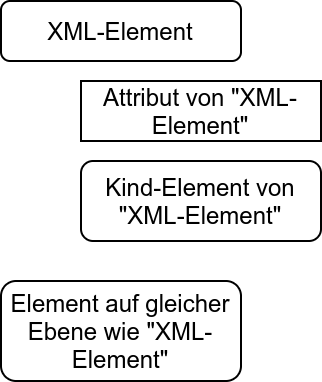
\includegraphics[width=.30\textwidth]{./img/legend.png}
			\caption{Legende für die folgenden Grafiken im Mapping}
			\label{fig:legend}
\end{figure}

\section{Operational Data Model}
\label{m:odm}

Das Operational Data Model (ODM) ist einer der Standards, welcher von CDISC entwickelt wurde, um den gesamten Zyklus einer Studie in ihren verschiedensten Formen zu standardisieren.
Es dient dazu, sowohl Metadaten als auch klinische Daten einer Studie zu erfassen. Auch administrative Daten sind im Standard enthalten.
ODM ist unabhängig von spezifischen Firmen und Plattformen und daher gut zum Austausch zwischen verschiedensten Werkzeugen und Gruppierungen geeignet.
Bereits 2006 hat ODM im internationalen Raum Anklang gefunden, in Deutschland allerdings noch nicht\cite{odm_art}.
Das ändert sich mittlerweile, das IMI der WWU zum Beispiel nutzt das Format bereits in mehreren Werkzeugen.
In dieser Arbeit wird Version \jv{1.3.2} genutzt.

\subsection{Aufbau}

Zuerst sollte angemerkt werden, dass hier nicht alle Elemente, die im ODM-Standard definiert sind, vorgestellt werden. Das hat sowohl Zeit- als auch Platzgründe, weiterhin werden viele Elemente für die Abbildung von LimeSurvey nicht gebraucht.
Eine vollständige Liste kann in der Dokumentation von ODM gefunden werden\cite{odm}.
Für diese Arbeit sind besonders zwei Teile des ODM Standards relevant: Die \el{Study} und die \el{ClinicalData}.
Weiterhin gibt es noch \el{AdminData}, \el{ReferenceData} und \el{Association}.
Grundlegend werden andere Elemente mittels einer OID referenziert, ein Attribut, welches jedes Element besitzt, das man referenzieren kann.

\subsubsection{Study}

Eine Studie hat globale Variablen und grundlegende Definitionen.
Weiterhin gibt es die \el{MetaDataVersion}, wo die Struktur der Umfrage festgelegt wird.
In der einer Version der Metadaten sind alle Elemente in Referenzen und Definitionen aufgeteilt, wobei die Referenzen immer zuerst im nächst \enquote{höhergelegenen} Element vorkommen.

Das Basiselement einer Studie ist das \el{Protocol}.
Dies enthält Elemente des Typs \el{StudyEventRef}.
Dann folgen Elemente des Typs \el{StudyEventDef}, welche wiederum Referenzen auf Elemente des Typs \el{FormDef} beinhalten.
Dieses Schema setzt sich noch mit den Elementen \el{ItemGroupDef} und \el{ItemDef} fort.
In \cref{fig:odm_ex} ist das Konzept noch einmal visualisiert.

\begin{figure}[h]
			\centering
			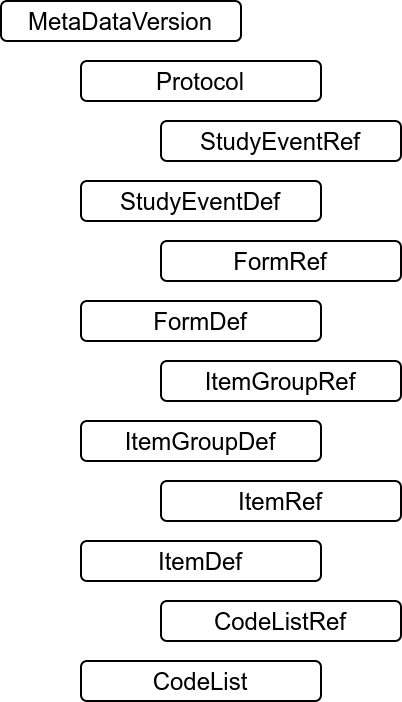
\includegraphics[width=.40\textwidth]{./img/met_odm.png}
			\caption{Die Struktur aus Referenzen und Definitionen in ODM}
			\label{fig:odm_ex}
\end{figure}

Als weitere Elemente gibt es noch die \el{CodeList} und die \el{Condition}.
In einer \el{CodeList} werden Antwortmöglichkeiten festgehalten, welche auf eine Frage (Element des Typs \el{ItemDef}) gegeben werden können.
Dabei gibt es zwei Arten von CodeLists, die simple und die komplexe.
Die simple Liste besteht aus \el{EnumeratedItems}, wo die Antwortmöglichkeit in dem Attribut \el{CodedValue} angegeben ist.
In den klinischen Daten wird als Antwort dann dieser codierte Wert stehen.
Die komplexe Liste hat dieses Attribut ebenfalls, in Elementen des Typs \el{CodeListItem}. Es ist auch als Antwort angegeben, aber die tatsächliche Antwortmöglichkeit ist der Text von \el{CodeListItem/Decode/TranslatedText}.

\el{ItemDef} enthält ein Element \el{Question}, in welchem eine Frage festgehalten wird.
Mit \el{ConditionDef} kann eine Bedingung festgelegt werden.
Eine Bedingung hat ein Kind-Element \el{FormalExpression}, dessen Text die Bedingung selber enthält.
Das Attribut \el{Context} gibt an, in welcher Sprache die Bedingung verfasst wurde.
Referenziert eine Frage eine Bedingung und evaluiert der Ausdruck zu \enquote{true}, wird die Frage nicht angezeigt.

\subsubsection{ClinicalData}

In der \el{ClinicalData} gibt es für jeden Teilnehmer der Studie ein Element des Typs \el{SubjectData}.
Ab hier ist dann die Stuktur der Studie abgebildet, wobei die \el{ItemData} das unterste Element ist und die Antwort auf eine Frage beinhaltet.

\section{Syntaxerweiterung des Instituts für Medizinische Infomatik}

ODM besitzt eine sehr lose Definition dessen, was als Bedingung gilt. Daher kann man eine extra Syntax/Sprache angeben, in welcher die Bedingung verfasst ist.
Das Institut für Medizinische Informatik der WWU (IMI) hat in einem internen Dokument eine eigene Syntax für Bedingungen entwickelt.
Die Antwort auf eine Frage wird mit dem folgenden Ausdruck referenziert: 

\reg{SE-\{SeOID\}/F-\{FOID\}/IG-\{IGOID\}/I-\{IOID\}}

\noindent wobei entsprechende OIDs eingesetzt werden, sodass die Frage eindeutig identifiziert werden kann.
Diese Selektoren werden wie Variablen in der sh-Syntax mit einem Dollarsymbol und runden Klammern umschlossen.
Durch Angabe des ganzen Pfades wird sichergestellt, dass die Referenz eindeutig ist. Auch eine bestimmte Wiederholung kann angegeben werden.
Sonst gibt es logische Operatoren wie \enquote{==, !=, <=, >=, AND, OR, NOT, IN,...} und mathematische Operatoren wie \enquote{+, -, *, /, MIN, MAX, SUM, MEDIAN, MEAN,...}.

\section{dom4j}

\jv{dom4j} ist eine API, welche die bestehenden Funktionen der \jv{javax}-Bibliothek abstrahiert und so wesentlich simplere Wege bietet, diese zu nutzen\cite{dom4j}.
Unter anderem ist es möglich, Elemente in einem XML-Dokument mittels XPath-Ausdrücken zu finden und DOM/SAX-Parser zu nutzen, um ein Dokument zu verarbeiten.
Auch ein \jv{XMLWriter} existiert, welcher unter anderem Standardelemente von XML automatisch an ein Dokument anhängt und das Format des Dokuments mittels eines einzeiligen Befehls so anpassen kann, dass es leicht für einen Menschen lesbar ist.
In dieser Arbeit wird Version \jv{1.6.1} verwendet.

\section{Reguläre Ausdrücke}

Reguläre Ausdrücke (RegEx) sind ein beliebtes Mittel, um in verschiedensten Anwendungsgebieten der Informatik Zeichenketten zu analysieren.
Die Hauptfunktion ist es, zu überprüfen, ob eine Zeichenkette einem bestimmten Format entspricht (bzw. ob es ein Match gibt).
Weitere Funktionen bestehen zum Beispiel darin, Teile der Zeichenkette zu extrahieren.\\

Es gibt eine eigene Syntax, in welcher ein Format spezifiziert werden kann\cite{regex101}.
Nennenswert hier ist, dass es verschiedene Syntaxen gibt, je nachdem in welcher Programmiersprache oder Umgebung man arbeitet.
Am bekanntesten und am weitesten verbreitet ist die \jv{Perl-Syntax}, Java hat jedoch eine leicht abweichende Syntax.
Der Anfang einer Zeichenkette wird mit \enquote{\textasciicircum} markiert, das Ende selbiger mit \enquote{\$}.
Weiterhin steht zum Beispiel \enquote{\textbackslash d} für eine beliebige Zahl (\textbackslash\textbackslash d in Java) oder \enquote{.} für jedes beliebige Zeichen.
Dann gibt es Quantoren, mit denen die Häufigkeit eines Ausdrucks bestimmt werden kann.
Sie stehen hinter den Ausdrücken, deren Häufigkeit sie bestimmen.
Dabei steht \enquote{?} für Null oder ein Vorkommnis, \enquote{*} für beliebig viele und \enquote{+} für mindestens ein Vorkommen.
In eckigen Klammern können Zeichen angegeben werden, welche gematcht werden sollen. So verlangt \enquote{[abc]} zum Beispiel, dass ein Zeichen an einer entsprechenden Stelle a, b oder c sein muss.\\

Es gibt auch \jv{Capture Groups}. Hiermit kann man, nachdem ein Match gefunden wurde, einen Teil der Zeichenkette erhalten, welcher dem Muster in der Capture Group entspricht. Diese wird mit runden Klammern markiert.

Dazu ein Beispiel: Man hat den Ausdruck \enquote{X(\textbackslash d+)X}, es wird also verlangt, dass die Zeichenkette mit einem \jv{X} beginnen muss, dann mindestens eine Ziffer hat und auf einem \jv{X} endet. 
Zusätzlich hat man noch die Zeichenkette \enquote{X0135X}, diese stimmt mit dem Format des Ausdrucks überein.
Durch Zugriff auf die Gruppe kann man nun die Zeichenkette \enquote{0135} erhalten.

In Java sieht der Einsatz von regulären Ausdrücken so aus:
Als erstes wird ein Ausdruck erstellt. Dazu dient in Java die Klasse \jv{Pattern}:
\reg{Pattern p = Pattern.compile("\{PATTERN\}");}
\noindent Als nächstes wird die Zeichenkette angegeben, die überprüft werden soll:
\reg{Matcher m = p.matcher("\{STRING\}");}
\noindent Nun wird die Methode \jv{find} der Klasse \jv{Matcher} aufgerufen, welche prüft, ob die Zeichenkette dem Ausdruck entspricht.
\reg{m.find();}
\noindent Zuletzt kann man auf alle \jv{Capture Groups} zugreifen, dazu dient die Methode \jv{group}:
\reg{m.group(\{GRUPPENNUMMER\});}
